\documentclass{article}
\usepackage{graphicx}
\graphicspath{{./figs/}}{}
\usepackage{listings}
\title{
HLS-Assignment 4
}
\begin{document}
\maketitle
\hfill \textbf{Sampath Govardhan} \\
\null \hfill \textbf{FWC22071}\\

\section{Problem Statement}
\begin{lstlisting}
Design a basic integer ALU unit in HLS that takes 3 inputs: Two 8bit 
operands and one appropriately sized operator. The permitted operations 
are ADD, SUB, MUL, DIV, AND, OR and XOR. Use AXI-S ports for all I/O 
ports.The design should be pipelined.
\end{lstlisting}
\vspace{10cm}


\section{Design Code}
\begin{lstlisting}
#include <iostream>
#include "ap_int.h"

typedef ap_int<8> in;
typedef ap_uint<3> op;
typedef ap_int<16> out;

void cal(in a, in b, op c, out *d)
{
#pragma HLS INTERFACE axis register both port=a
#pragma HLS INTERFACE axis register both port=b
#pragma HLS INTERFACE axis register both port=c
#pragma HLS INTERFACE axis register both port=d
#pragma HLS PIPELINE

 switch(c){
 case 0: *d=a+b; break;
 case 1: *d=a-b; break;
 case 2: *d=a*b; break;
 case 3: *d=a/b; break;
 case 4: *d=a&b; break;
 case 5: *d=a|b; break;
 case 6: *d=a^b; break;
 default: break;
 }

}



\end{lstlisting}
\vspace{5cm}


\section{Test Bench Code}
\begin{lstlisting}
#include <fstream>
#include <iostream>
#include "ap_int.h"
using namespace std;

typedef ap_int<8> in;
typedef ap_uint<3> op;
typedef ap_int<16> out;

void cal(in a, in b, op c, out *d);

int main() {
    in m,n;
    op o;
    out ref,res;
    bool q;

    ifstream fo("in.dat");
    ofstream fi("out.dat");

    for (int i=0;i<9;i++){
    	fo>>o>>m>>n>>ref;
    	cal(m,n,o,&res);
         if (res==ref)
         {
    	fi<<" "<<res<<" "<<"Pass"<<"\n";
        }
         else {
    	q=1;
    	fi<<" "<<res<<" "<<"Fail"<<"\n";
          }
    }
   fo.close();
   fi.close();
   if (q!=1){
	   cout<<"ALL THE TEST CASES ARE PASSED!";
   }
   else{
	   cout<<"ALL THE TEST CASES ARE NOT PASSED!";
   }
   return 0;
}


\end{lstlisting}
\vspace{5cm}
\section{Generating Input file}
\begin{lstlisting}
#include <stdio.h>
#include <stdlib.h>

int main() {
    int a,b;
    int op;
    int r;
    FILE *fp;
    fp=fopen("in.dat","w");
    for (int i=1;i<10;i++){
    a=i;
    b=i*3;
    op=i%7;
     switch(op){
 case 0: r=a+b; break;
 case 1: r=a-b; break;
 case 2: r=a*b; break;
 case 3: r=a/b; break;
 case 4: r=a&b; break;
 case 5: r=a|b; break;
 case 6: r=a^b; break;
 default: break;
 }
    
   
   
   fprintf(fp,"%d  %d  %d  %d\n",op,a,b,r);
    }
   fclose(fp);

    return 0;
}
\end{lstlisting}
\section{in.dat file}
\begin{lstlisting}
1  1  3  -2
2  2  6  12
3  3  9  0
4  4  12  4
5  5  15  15
6  6  18  20
0  7  21  28
1  8  24  -16
2  9  27  243
\end{lstlisting}
\section{out.dat file}
\begin{lstlisting}
 -2 Pass
 12 Pass
 0 Pass
 4 Pass
 15 Pass
 20 Pass
 28 Pass
 -16 Pass
 243 Pass
\end{lstlisting}
\vspace{5cm}


\section{C Simulation Output}
\begin{lstlisting}
INFO: [SIM 2] *************** CSIM start ***************
INFO: [SIM 4] CSIM will launch GCC as the compiler.
   Compiling ../../../../func_sized.cpp in debug mode
   Generating csim.exe
ALL THE TEST CASES ARE PASSED!
INFO: [SIM 1] CSim done with 0 errors.
INFO: [SIM 3] *************** CSIM finish ***************

\end{lstlisting}
\vspace{15cm}


\section{HLS Resource Consumption}
\vspace{3cm}
\begin{figure}[h]
    \centering
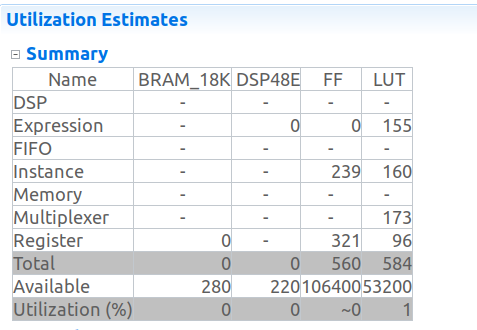
\includegraphics[width=\columnwidth]{1.png}
    \caption{Resource Consumption}
    \label{fig:my_label}
\end{figure}

\vspace{5cm}


\section{HLS Timing Report}
\vspace{1cm}
\begin{figure}[h]
    \centering
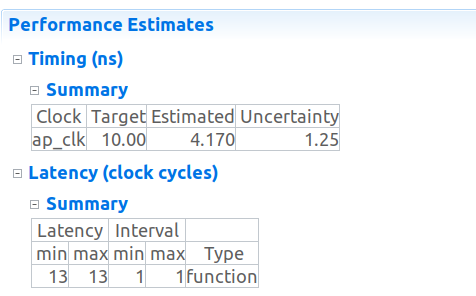
\includegraphics[width=\columnwidth]{figs/2.png}
    \caption{Timing Report}
    \label{fig:my_label}
\end{figure}

\vspace{10cm}


\section{Interfaces Report}
\vspace{1cm}
\begin{figure}[h]
    \centering
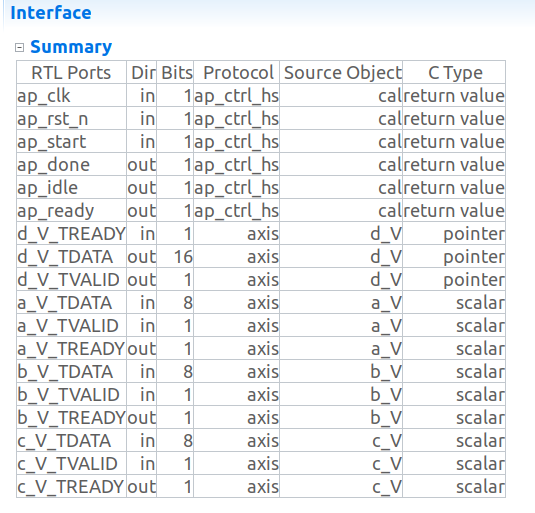
\includegraphics[width=\columnwidth]{figs/3.png}
    \caption{Interface Summmary}
    \label{fig:my_label}
\end{figure}
\vspace{5cm}


\section{C/RTL Cosimulation Output}
\vspace{1cm}
\begin{lstlisting}


Starting C/RTL cosimulation ...
/tools/Xilinx/Vivado/2018.3/bin/vivado_hls /home/sam-admin/Xilinx/HLS/func_sized/proj_func_sized/solution1/cosim.tcl
INFO: [HLS 200-10] Running '/tools/Xilinx/Vivado/2018.3/bin/unwrapped/lnx64.o/vivado_hls'
INFO: [HLS 200-10] For user 'sam-admin' on host 'sampaths-lappie' (Linux_x86_64 version 5.19.0-35-generic) on Fri Mar 24 15:23:02 IST 2023
INFO: [HLS 200-10] On os Ubuntu 22.04.2 LTS
INFO: [HLS 200-10] In directory '/home/sam-admin/Xilinx/HLS/func_sized'
INFO: [HLS 200-10] Opening project '/home/sam-admin/Xilinx/HLS/func_sized/proj_func_sized'.
INFO: [HLS 200-10] Opening solution '/home/sam-admin/Xilinx/HLS/func_sized/proj_func_sized/solution1'.
INFO: [SYN 201-201] Setting up clock 'default' with a period of 10ns.
INFO: [HLS 200-10] Setting target device to 'xc7z020clg484-1'
INFO: [COSIM 212-47] Using XSIM for RTL simulation.
INFO: [COSIM 212-14] Instrumenting C test bench ...
WARNING: [COSIM 212-75] Fifo port 'd_V' has a default depth of 1. Insufficient depth may cause simulation mismatch or freeze. Please specify the depth in 'set_directive_interface' using the option '-depth'.
   Build using "/tools/Xilinx/Vivado/2018.3/tps/lnx64/gcc-6.2.0/bin/g++"
   Compiling apatb_cal.cpp
   Compiling func_sized.cpp_pre.cpp.tb.cpp
   Compiling func_sized_test.cpp_pre.cpp.tb.cpp
   Generating cosim.tv.exe
INFO: [COSIM 212-302] Starting C TB testing ... 
ALL THE TEST CASES ARE PASSED!INFO: [COSIM 212-333] Generating C post check test bench ...
INFO: [COSIM 212-12] Generating RTL test bench ...
INFO: [COSIM 212-323] Starting verilog simulation. 
INFO: [COSIM 212-15] Starting XSIM ...
INFO: [XSIM 43-3496] Using init file passed via -initfile option "/tools/Xilinx/Vivado/2018.3/data/xsim/ip/xsim_ip.ini".
Vivado Simulator 2018.3
Copyright 1986-1999, 2001-2018 Xilinx, Inc. All Rights Reserved.
Running: /tools/Xilinx/Vivado/2018.3/bin/unwrapped/lnx64.o/xelab xil_defaultlib.apatb_cal_top glbl -prj cal.prj -L smartconnect_v1_0 -L axi_protocol_checker_v1_1_12 -L axi_protocol_checker_v1_1_13 -L axis_protocol_checker_v1_1_11 -L axis_protocol_checker_v1_1_12 -L xil_defaultlib -L unisims_ver -L xpm --initfile /tools/Xilinx/Vivado/2018.3/data/xsim/ip/xsim_ip.ini --lib ieee_proposed=./ieee_proposed -s cal 
Multi-threading is on. Using 6 slave threads.
WARNING: [XSIM 43-3431] One or more environment variables have been detected which affect the operation of the C compiler. These are typically not set in standard installations and are not tested by Xilinx, however they may be appropriate for your system, so the flow will attempt to continue.  If errors occur, try running xelab with the "-mt off -v 1" switches to see more information from the C compiler. The following environment variables have been detected:
    LIBRARY_PATH
INFO: [VRFC 10-2263] Analyzing SystemVerilog file "/home/sam-admin/Xilinx/HLS/func_sized/proj_func_sized/solution1/sim/verilog/glbl.v" into library work
INFO: [VRFC 10-311] analyzing module glbl
INFO: [VRFC 10-2263] Analyzing SystemVerilog file "/home/sam-admin/Xilinx/HLS/func_sized/proj_func_sized/solution1/sim/verilog/cal_sdiv_9s_8s_9_13_1.v" into library xil_defaultlib
INFO: [VRFC 10-311] analyzing module cal_sdiv_9s_8s_9_13_1_div_u
INFO: [VRFC 10-311] analyzing module cal_sdiv_9s_8s_9_13_1_div
INFO: [VRFC 10-311] analyzing module cal_sdiv_9s_8s_9_13_1
INFO: [VRFC 10-2263] Analyzing SystemVerilog file "/home/sam-admin/Xilinx/HLS/func_sized/proj_func_sized/solution1/sim/verilog/cal.autotb.v" into library xil_defaultlib
INFO: [VRFC 10-311] analyzing module apatb_cal_top
INFO: [VRFC 10-2263] Analyzing SystemVerilog file "/home/sam-admin/Xilinx/HLS/func_sized/proj_func_sized/solution1/sim/verilog/AESL_axi_s_c_V.v" into library xil_defaultlib
INFO: [VRFC 10-311] analyzing module AESL_axi_s_c_V
INFO: [VRFC 10-2263] Analyzing SystemVerilog file "/home/sam-admin/Xilinx/HLS/func_sized/proj_func_sized/solution1/sim/verilog/AESL_axi_s_b_V.v" into library xil_defaultlib
INFO: [VRFC 10-311] analyzing module AESL_axi_s_b_V
INFO: [VRFC 10-2263] Analyzing SystemVerilog file "/home/sam-admin/Xilinx/HLS/func_sized/proj_func_sized/solution1/sim/verilog/AESL_axi_s_a_V.v" into library xil_defaultlib
INFO: [VRFC 10-311] analyzing module AESL_axi_s_a_V
INFO: [VRFC 10-2263] Analyzing SystemVerilog file "/home/sam-admin/Xilinx/HLS/func_sized/proj_func_sized/solution1/sim/verilog/AESL_axi_s_d_V.v" into library xil_defaultlib
INFO: [VRFC 10-311] analyzing module AESL_axi_s_d_V
INFO: [VRFC 10-2263] Analyzing SystemVerilog file "/home/sam-admin/Xilinx/HLS/func_sized/proj_func_sized/solution1/sim/verilog/AESL_fifo.v" into library xil_defaultlib
INFO: [VRFC 10-311] analyzing module fifo
INFO: [VRFC 10-2263] Analyzing SystemVerilog file "/home/sam-admin/Xilinx/HLS/func_sized/proj_func_sized/solution1/sim/verilog/cal.v" into library xil_defaultlib
INFO: [VRFC 10-311] analyzing module cal
Starting static elaboration
Completed static elaboration
Starting simulation data flow analysis
Completed simulation data flow analysis
Time Resolution for simulation is 1ps
Compiling module xil_defaultlib.cal_sdiv_9s_8s_9_13_1_div_u(in0_...
Compiling module xil_defaultlib.cal_sdiv_9s_8s_9_13_1_div(in0_WI...
Compiling module xil_defaultlib.cal_sdiv_9s_8s_9_13_1(ID=1,NUM_S...
Compiling module xil_defaultlib.cal
Compiling module xil_defaultlib.fifo(DEPTH=1)
Compiling module xil_defaultlib.AESL_axi_s_a_V
Compiling module xil_defaultlib.AESL_axi_s_b_V
Compiling module xil_defaultlib.AESL_axi_s_c_V
Compiling module xil_defaultlib.fifo(DEPTH=1,WIDTH=16)
Compiling module xil_defaultlib.AESL_axi_s_d_V
Compiling module xil_defaultlib.apatb_cal_top
Compiling module work.glbl
Built simulation snapshot cal


****** Webtalk v2018.3 (64-bit)
  **** SW Build 2405991 on Thu Dec  6 23:36:41 MST 2018
  **** IP Build 2404404 on Fri Dec  7 01:43:56 MST 2018
    ** Copyright 1986-2018 Xilinx, Inc. All Rights Reserved.


source /home/sam-admin/Xilinx/HLS/func_sized/proj_func_sized/solution1/sim/verilog/xsim.dir/cal/webtalk/xsim_webtalk.tcl -notrace
INFO: [Common 17-206] Exiting Webtalk at Fri Mar 24 15:23:47 2023...


****** xsim v2018.3 (64-bit)
  **** SW Build 2405991 on Thu Dec  6 23:36:41 MST 2018
  **** IP Build 2404404 on Fri Dec  7 01:43:56 MST 2018
    ** Copyright 1986-2018 Xilinx, Inc. All Rights Reserved.


source xsim.dir/cal/xsim_script.tcl
# xsim {cal} -autoloadwcfg -tclbatch {cal.tcl}
Vivado Simulator 2018.3
Time resolution is 1 ps
source cal.tcl
## run all
////////////////////////////////////////////////////////////////////////////////////
// Inter-Transaction Progress: Completed Transaction / Total Transaction
// Intra-Transaction Progress: Measured Latency / Latency Estimation * 100%
//
// RTL Simulation : "Inter-Transaction Progress" ["Intra-Transaction Progress"] @ "Simulation Time"
////////////////////////////////////////////////////////////////////////////////////
// RTL Simulation : 0 / 9 [0.00%] @ "125000"
// RTL Simulation : 1 / 9 [192.31%] @ "415000"
// RTL Simulation : 2 / 9 [192.31%] @ "435000"
// RTL Simulation : 3 / 9 [192.31%] @ "455000"
// RTL Simulation : 4 / 9 [192.31%] @ "475000"
// RTL Simulation : 5 / 9 [192.31%] @ "495000"
// RTL Simulation : 6 / 9 [192.31%] @ "515000"
// RTL Simulation : 7 / 9 [192.31%] @ "535000"
// RTL Simulation : 8 / 9 [192.31%] @ "555000"
// RTL Simulation : 9 / 9 [100.00%] @ "575000"
////////////////////////////////////////////////////////////////////////////////////
$finish called at time : 615 ns : File "/home/sam-admin/Xilinx/HLS/func_sized/proj_func_sized/solution1/sim/verilog/cal.autotb.v" Line 326
## quit
INFO: [Common 17-206] Exiting xsim at Fri Mar 24 15:24:04 2023...
INFO: [COSIM 212-316] Starting C post checking ...
ALL THE TEST CASES ARE PASSED!INFO: [COSIM 212-1000] *** C/RTL co-simulation finished: PASS ***
Finished C/RTL cosimulation.



\end{lstlisting}
\vspace{5cm}


\section{C/RTL Cosimulation Report}
\vspace{1cm}
\begin{figure}[h]
    \centering
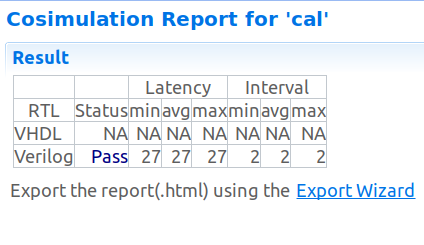
\includegraphics[width=\columnwidth]{figs/4.png}
    \caption{Cosimulation Report}
    \label{fig:my_label}
\end{figure}
\end{document}
